\documentclass[a4paper,12pt]{article}

\usepackage[utf8]{inputenc}
\usepackage[english]{babel}
\usepackage{natbib}
\usepackage[T1]{fontenc}
\usepackage{setspace}
\usepackage{graphicx}
\usepackage{hyperref}
\usepackage{csquotes}


\title{Literature Review}
\author{Joshua Bridge \\14032908 \\joshua.m.bridge@stu.mmu.ac.uk}

\pagestyle{headings}

\begin{document}

\maketitle


\tableofcontents

\listoffigures

\doublespacing

\subsection{Introduction}
  In order to understand the background of the technology involved in this project, it is necessary to complete a significant review into the current and past literature. This will help form a basis of knowledge from which the future development and analysis of the proposed system will utilise and build upon. This research will be vital in order to make use of the most optimal technology for any given problem.

  The following review will be an investigation into the current knowledge of the three major components of the proposed system, which are as follows:

  \begin{itemize}
    \item The recommendation system.
    \item The image-filter generation system.
    \item The web-based user interface.
  \end{itemize}

\section{Recommendation systems}
  As defined in \cite{ricci2011introduction}, recommending content is a problem which involves attempting to predict what a user may desire at any given time when using a system. In the ‘internet era’ applications of this are far-reaching, such as recommending products on Amazon.com \cite{linden2003amazon}. Recommendation systems are a popular topic due to the \textquote{abundance of practical applications that help users to deal with information overload and provide personalized recommendations, content, and services to them} \citep{adomavicius2005toward}.

  \cite{jannach2010recommender} describe three different methods for giving recommendations: Knowledge-based (inc. Collaborative), Content-based, and Hybrid.

  \subsection{Knowledge-based / Collaborative recommendation}
    When using an online streaming platform that serves video content such as Netflix or YouTube, a user will visit their site looking for something to watch. The problem faced by these sites is trying to find content that the user hasn't seen before, but will align with the user's interests enough to make them want to watch it.
    The information needed to carry out such a prediction can include the users history of interaction with the system, from which preference can be extrapolated (a.k.a. ‘metadata’). If there is not enough metadata about the user from which to extrapolate preference with reasonable certainty, then preference can be inferred from other users of the system - especially users with a similar predicted preference.

  \subsection{Content-based recommendation}

  \subsection{Hybrid recommendation}

    \subsubsection{Spotify - Discover Weekly}
      Discover Weekly is a playlist made every week for every user of Spotify. Instead of getting humans to curate a playlist for each and every user, an algorithm is used to try and find a set of songs which it predicts the user will like, but hasn't listened to before. As described by \cite{popper2015dw} it does this by mixing collaborative and content-based recommendation. The first is done by analysing every playlist ever made on spotify and determining their similarity to the playlists made by the user. The next step is looking for songs in those playlists that the user in question hasn't heard yet.

      \begin{figure}[ht]
        \centering
        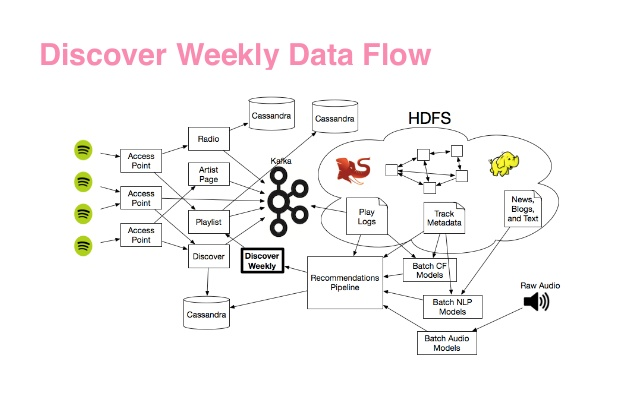
\includegraphics[width=\linewidth]{images/discoverweekly-dataflow}
        \caption[System component architecture of Spotify's ‘Discover Weekly’]{System component architecture of Spotify's ‘Discover Weekly’ \protect\citep{johnson2015dw}}
        \label{fig:discoverweekly-dataflow}
      \end{figure}

      The second, more complicated part of this process is the content-based recommendation. Spotify's algorithms actually analyse the music data in several different ways to determine a users ‘taste’. The first is by defining the generes a user listens to, which it does by scanning music blogs for what genre a certain piece of music is described as being. Using this as a search, spotify can then look for other music in that genre to recommend. The arguably more complicated part of this process is the auditory analysis of raw music data. As shown in figure \ref{fig:discoverweekly-dataflow} the raw audio is converted into ‘batch audio models’ where they can be used as a basis for recommendations.

  \subsection{Machine learning recommendation}
  \subsection{Image classification in recommendations}

\section{Image-filter generation}

\section{Web-based user interface}

\section{Conclusion}

\newpage
\singlespacing

\bibliographystyle{agsm}
\bibliography{literature-review}


\end{document}
